\subsection{\texorpdfstring{Wjets background estimation in $\tauTau$ channel}{Wjets background estimation in tau-tau channel}}
\label{sect:bkgW}
\subsubsection{Method description}
As shown in table~\ref{tbl:cutflowtable}, the number of Wjets events surviving 
the selection cuts is found to be zero in \binone, which may suffer from the low statistics of the Wjets sample. In addition, we need to verify if the Wjets events are simulated well and agree with data.
 The statistical uncertainty on the yields for Wjets events can be improved by extracting 
the $\mttwo$ cut efficiency in a sample with more statistics. To make this sample, some cuts with small correlation on the search variable are 
relaxed. Various samples with different relaxed cuts are examined to check the idea of small correlation 
between search variable and relaxed cuts. In the next section, the validation of this method will be discussed.\\
When the cut efficiency for the $\mttwo$ variable is found, then it is multiplied by the Wjets 
yields before cutting on this variable. This means, according to table~\ref{tbl:cutflowtable}, the cut efficiency for 
$\mttwo$ found in a relaxed sample should be multiplied by 31.93 to get an 
estimate for the Wjets events in  \binone.\\

\subsubsection{Method validation}
The idea is to check the effect of three set of cuts independently, 
on the \mttwo cut efficiency in  \binone. 
Therefore, starting with a baseline selection cuts, defined as two 
medium-isolated opposite sign \Tau's, the $\mttwo$ cut 
efficiency is calculated, for those events passing and failing the following list of cuts (one-by-one)
\begin{itemize}
\item lepton veto
\item $\mindphifour>$ 1
\item Z veto 
\end{itemize}

In order to evaluate the systematics, the cut efficiencies from the scaled samples with 
up and down Tau Energy Scale (as the main source of systematics) are also evaluated.
To make these scaled samples, the four-vector of all tau objects 
are scaled up and down by 3\% and all $p_T$-related variables such as $E_T^{miss}$ 
and $M_{T2}$ are recalculated.\\
The final estimated Wjets events in \binone for nominal as well as up and down scaled samples 
can be found in figure~\ref{fig:wjets_1}.  
\begin{figure}[!Hhtb]
\centering
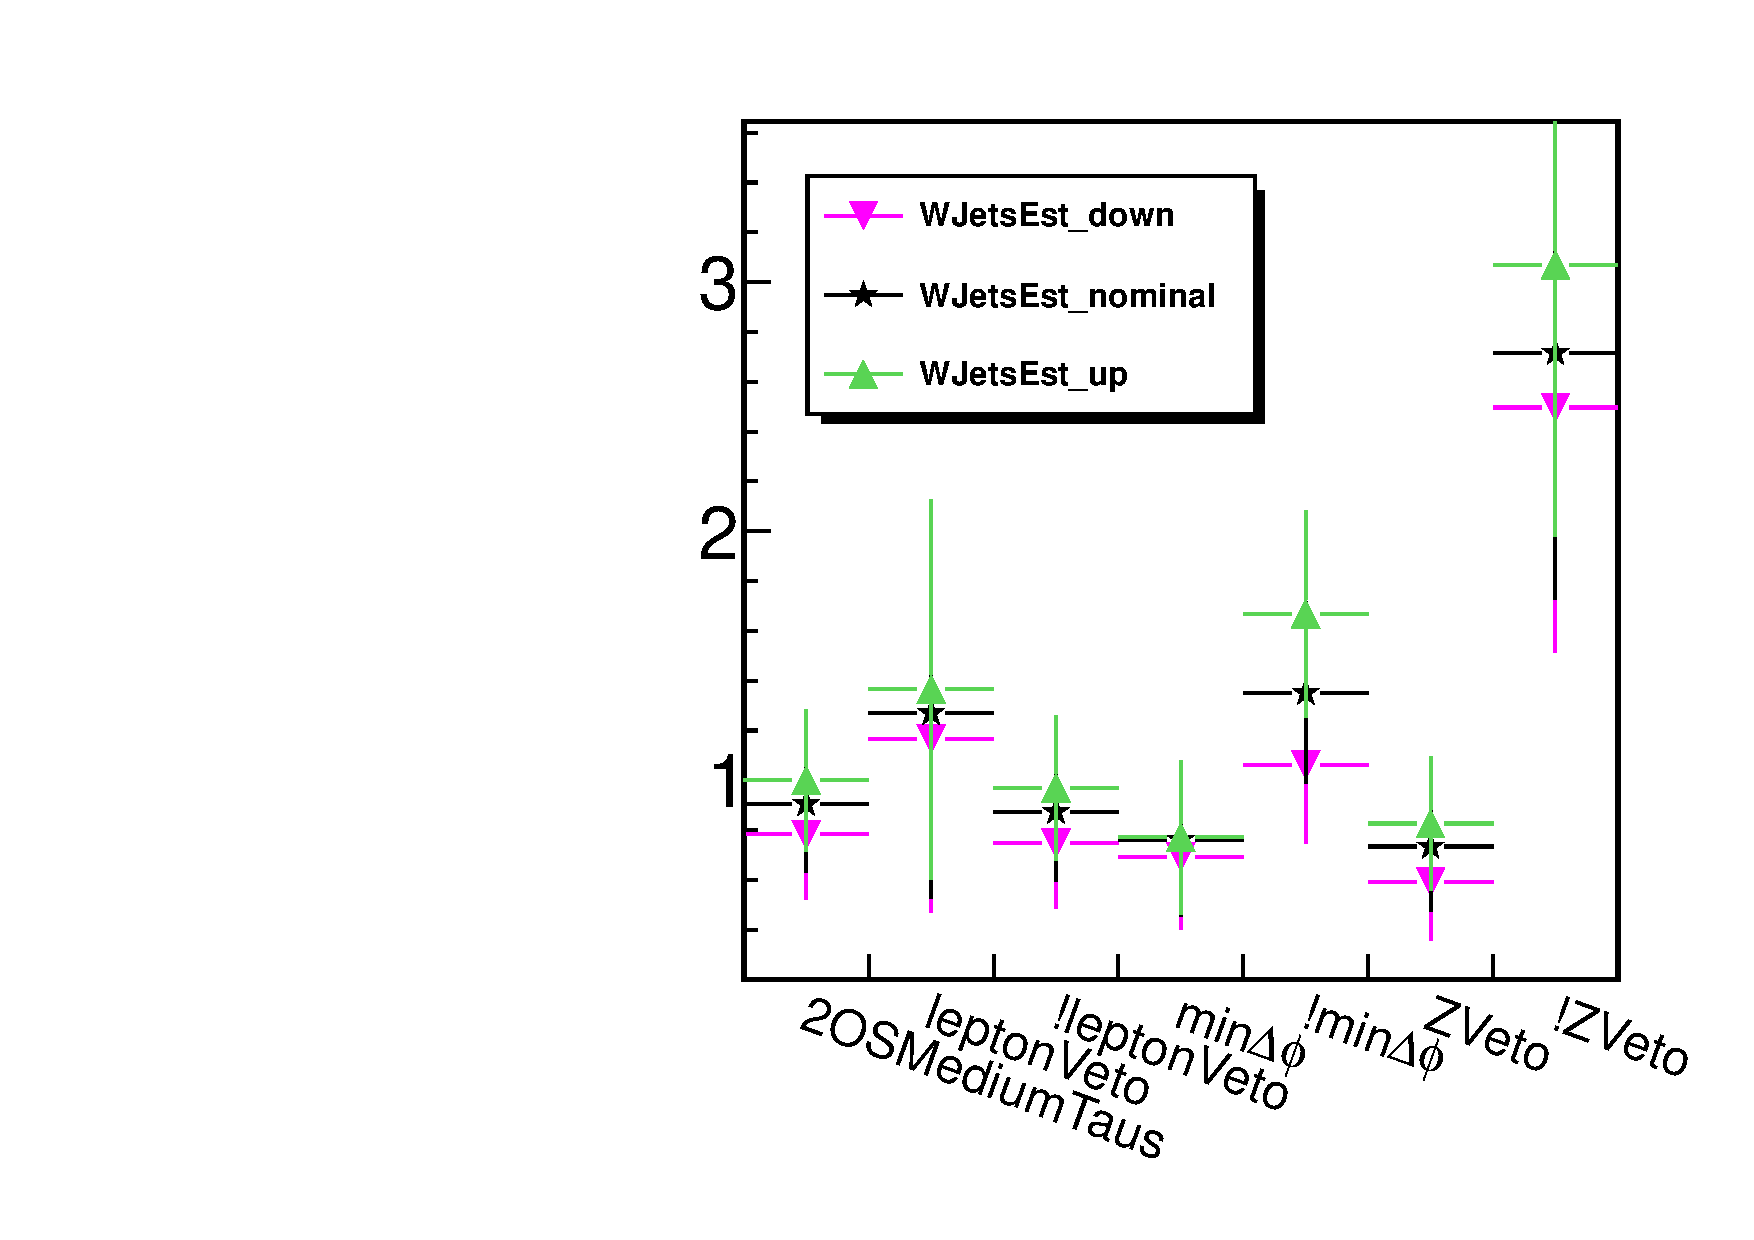
\includegraphics[angle=0,scale=0.35]{TauTauFigs/WJets_bin1.pdf}
\caption{The distribution of the final estimated Wjets events in \binone is shown in black. 
 The first bin of the histogram corresponds to the sample of events passing the baseline selection cuts. 
The next six bins correspond to the samples where passing and failing the 
list of cuts mentioned in the text, respectively. Also shown are the estimated Wjets events in up and down scaled samples to evaluate the systematics.}
\label{fig:wjets_1}
\end{figure}

Each of the three plots in figure~\ref{fig:wjets_1} are fitted with a pol0 function. The results are summarized in table~\ref{tbl:fitpars}.
\begin{table}[!Hhtb]
\begin{center}
\begin{tabular}{lc}
\hline\hline
  & Fit Parameters (pol0) \\
\hline\hline
WJetsEst\_down & 0.79 $\pm$ 0.12 \\
WJetsEst\_nominal & 0.93 $\pm$ 0.13 \\
WJetsEst\_up & 1.02 $\pm$ 0.13 \\
\hline\hline
\end{tabular}
\caption{The fit parameters obtained from Wjets estimation results in nominal, up and down scaled samples.}
\label{tbl:fitpars}
\end{center}
\end{table}

The systematics that can be assigned is the maximum variation of the up and down central values with 
respect to the nominal one. 

\subsubsection{MC validation for Wjets}
To verify that the MC has a good description of the Wjets events and it can be trusted for both shape and normalization, a data/MC comparison 
is done in a Wjets enriched sample. To enrich the sample, \muTau selection is done with the following modifications:
\begin{itemize}
\item $\mu$ and \Tau are same sign.
\item B-tagged jets with CSVL are vetoed.
\item \Tau isolation changed from Tight to Loose.
\end{itemize}
Figure \ref{fig:mt2_WValidation} 
\begin{figure}[!Hhtb]
\centering
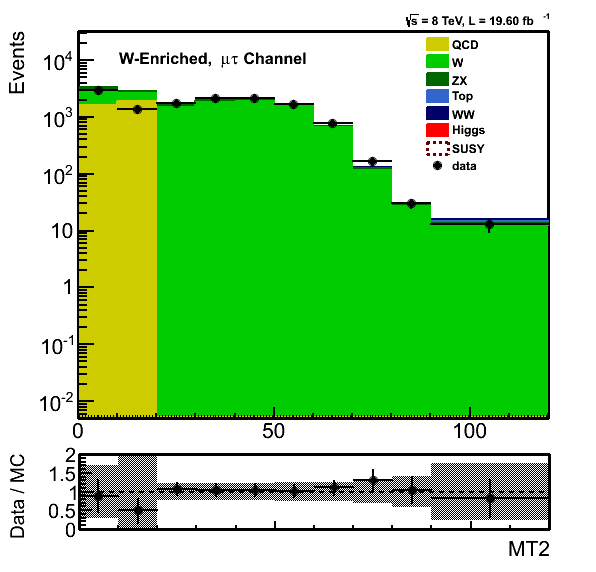
\includegraphics[angle=0,scale=0.35]{TauTauFigs/MT2_WValidation.png}
\caption{The \mttwo distribution in the W-Enriched region. Data and MC agree in both shape and normalization within the uncertainties.}
\label{fig:mt2_WValidation}
\end{figure}
shows the \mttwo distribution for the selected events. We use the range 40 $<\mttwo<$ 60 \GeV to find the normalization factor of the 
Wjets sample. In this range more than 90\% of the MC events are from the Wjets sample. 
All of the non-W MC events in this range are subtracted from 
the data in the same range. The result is compared with the MC prediction for the Wjets in this range. The k-factor for the Wjets sample is 
found to be 1.05 $\pm$ 0.13 which is compatible with 1 within the errors. To evaluate the uncertainty, 
all of the statistical uncertainties on data and MC are considered plus 25\% systematic uncertainty on the MC samples.

To validate the shape of the Wjets sample, we compare the ratio of events with \mttwo $>$ 90 \GeV and  \mttwo $>$ 40 \GeV in data and MC.
The procedures to find the Wjets in data and consider the uncertainties are exactly same as the procedures for extracting the normalization  
factor. This ratio is found to be 0.00213 $\pm$ 0.00086 in data and  0.0029 $\pm$ 0.0019 in MC. To take into account the difference between 
the two values, the MC prediction is corrected by the ratio of the two values and its uncertainty is also taken into account which is about 70\%. 
This uncertainty  is added to other systematic uncertainties of the estimation in quadrature.
A summary of the estimated Wjets events in \binone can be found in table~\ref{tbl:wjetsEstimation}. 
\begin{table}[!Hhtb]
\begin{center}
\begin{tabular}{lc}
\hline\hline
& Wjets Estimated Results\\
\hline
\binone & 0.69 $\pm$ 0.13 (stat.) $\pm$ 0.14 (sys. fit) $\pm$ 0.52 (sys. shape)\\
\hline\hline 
\end{tabular}
\caption{The Wjets estimation results in \binone. The systematics comes from the maximum 
variation of the estimation found from up and down scaled samples with respect to the nominal one.}
\label{tbl:wjetsEstimation}
\end{center}
\end{table}

As the simulation of Wjets events agrees well with data in the bulk of \mttwo, for the \bintwo, 
the expected number of Wjets from MC which is $0.43\pm0.4$ is trusted and is used.

